\section{Image Segmentation}

\begin{frame}{Trainingseingaben}
    \begin{figure}
        \centering
        \begin{subfigure}{0.495\textwidth}
            \centering
            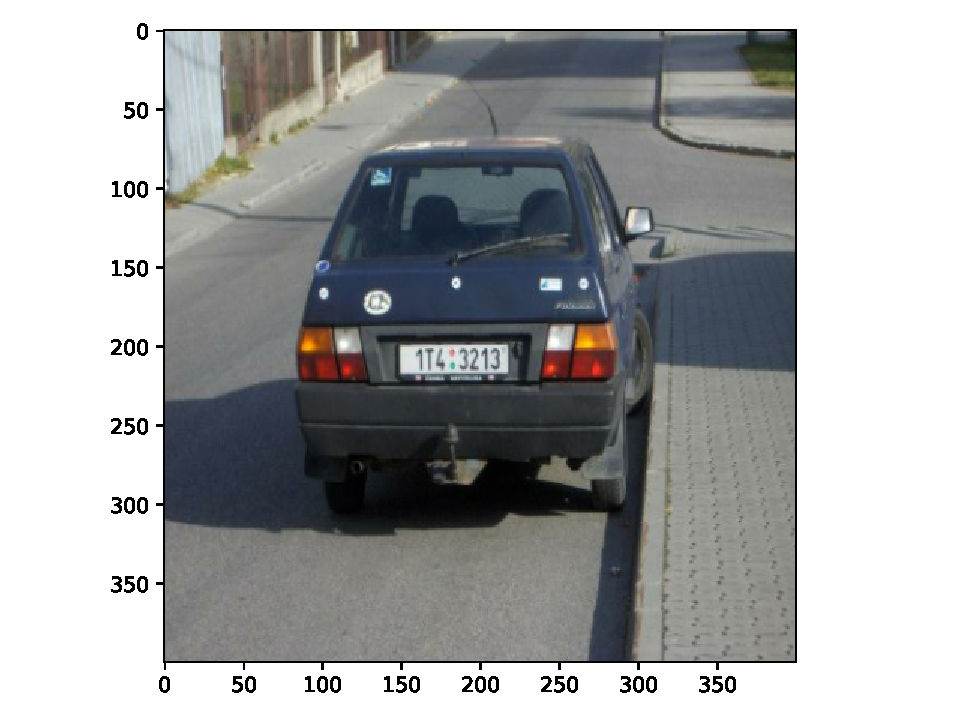
\includegraphics[width=\textwidth]{img/model_demo_1}
            \caption{Eingabe}
        \end{subfigure}
        \begin{subfigure}{0.495\textwidth}
            \centering
            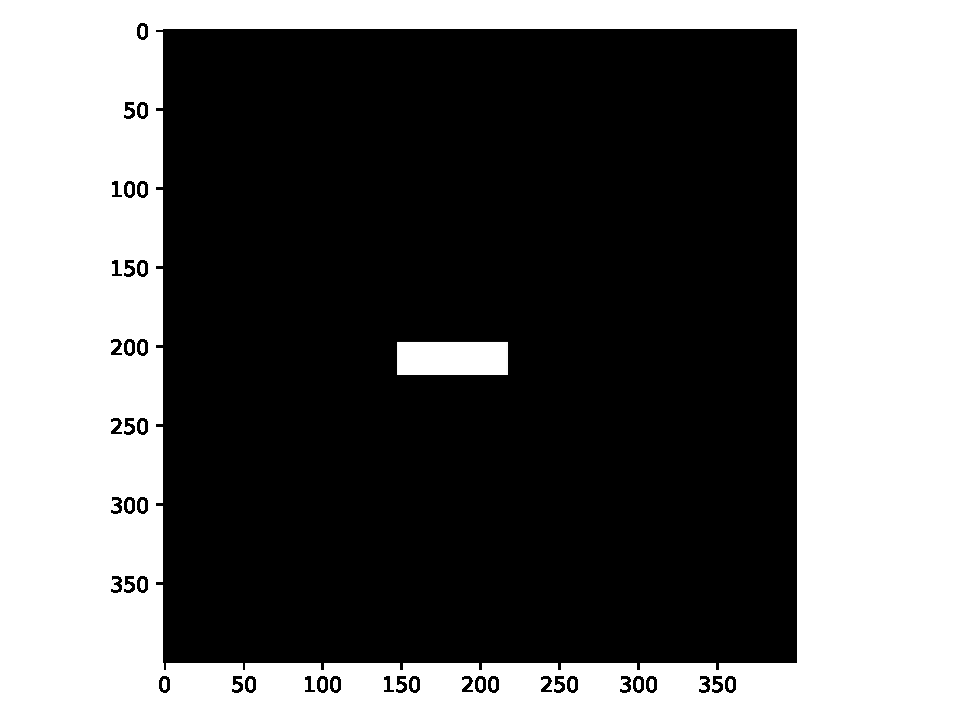
\includegraphics[width=\textwidth]{img/model_demo_2}
            \caption{Ziel}
        \end{subfigure}
    \end{figure}
\end{frame}

\begin{frame}{Modellarchitektur}
    \begin{figure}
        \centering
        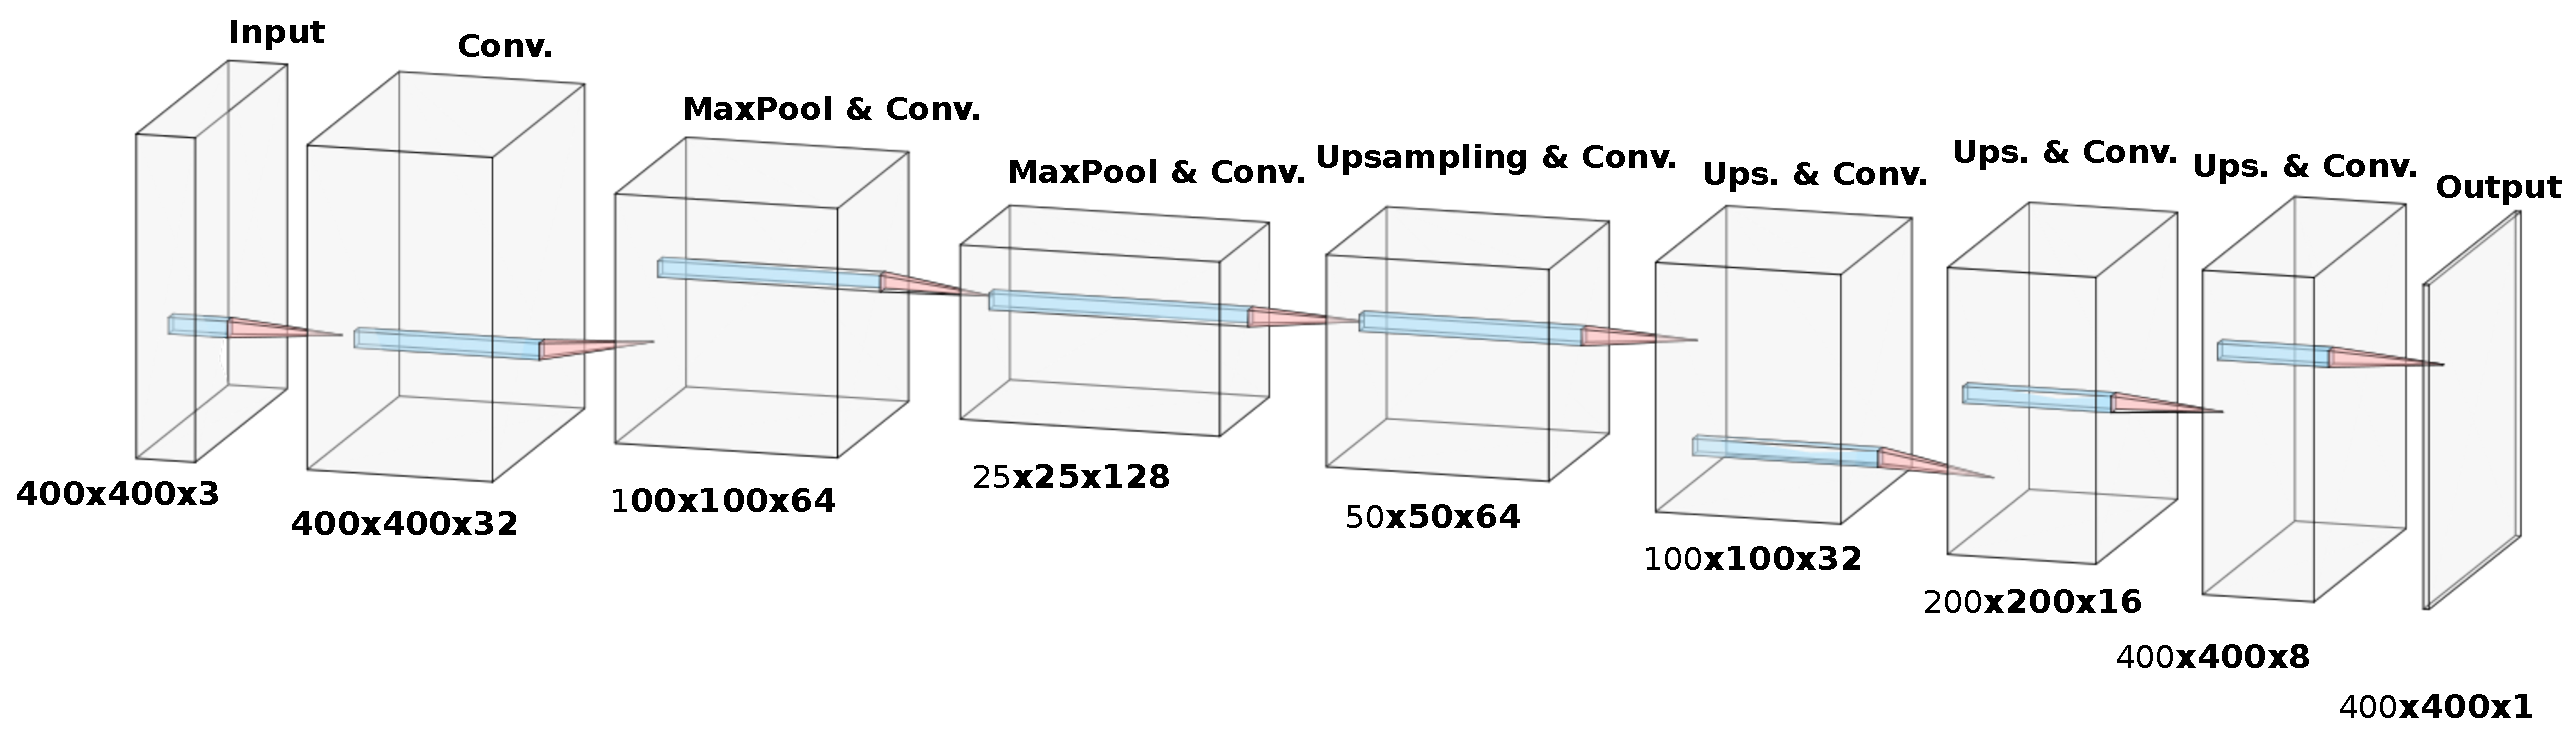
\includegraphics[width=\textwidth]{img/nn.pdf}
        \caption{Das Ergebnis nach wochenlangem Ausprobieren.}
    \end{figure}
\end{frame}

\begin{frame}{Modellvorhersage}
    \begin{figure}
        \centering
        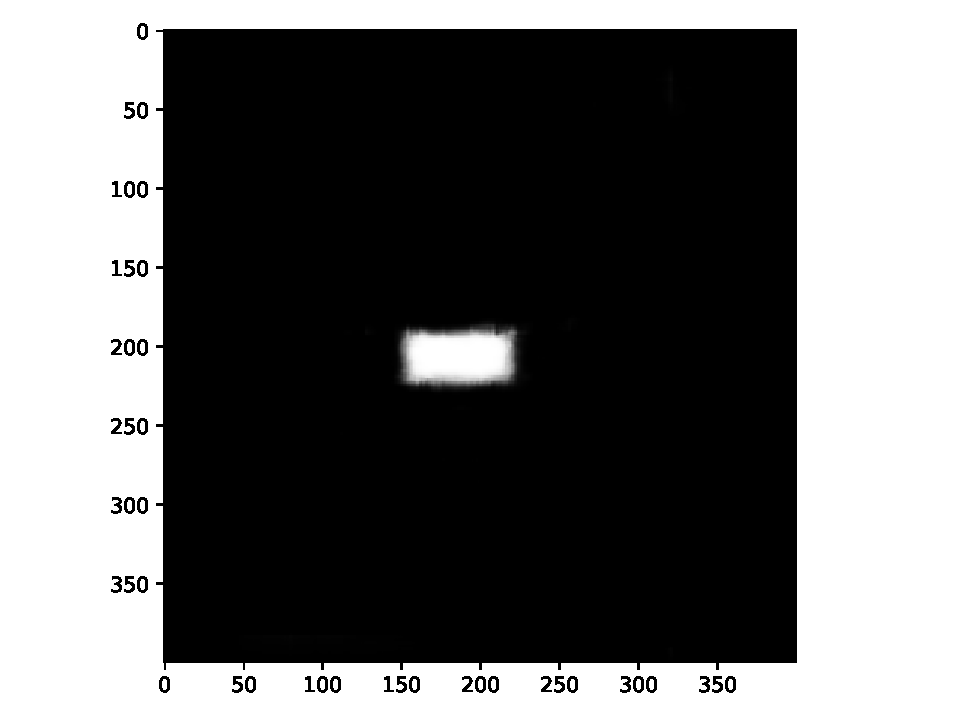
\includegraphics[width=0.9\textwidth]{img/model_demo_3}
    \end{figure}
\end{frame}

\begin{frame}{Schwellenwert}
    \begin{figure}
        \centering
        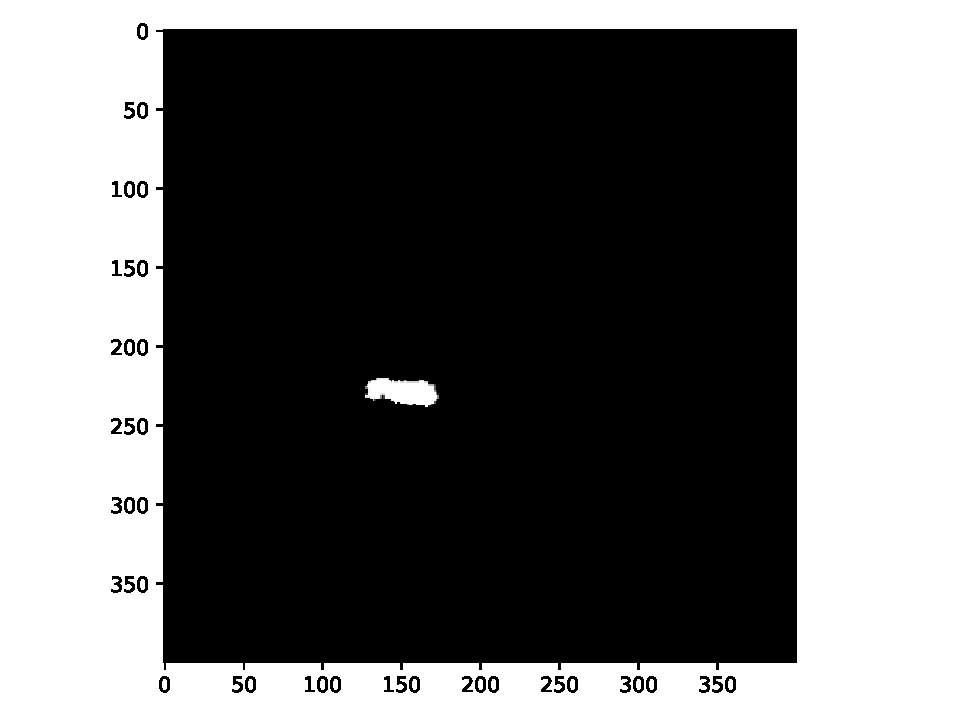
\includegraphics[width=0.9\textwidth]{img/model_demo_4}
    \end{figure}
\end{frame}

\begin{frame}{Umschlie{\ss}endes Rechteck}
    \begin{figure}
        \centering
        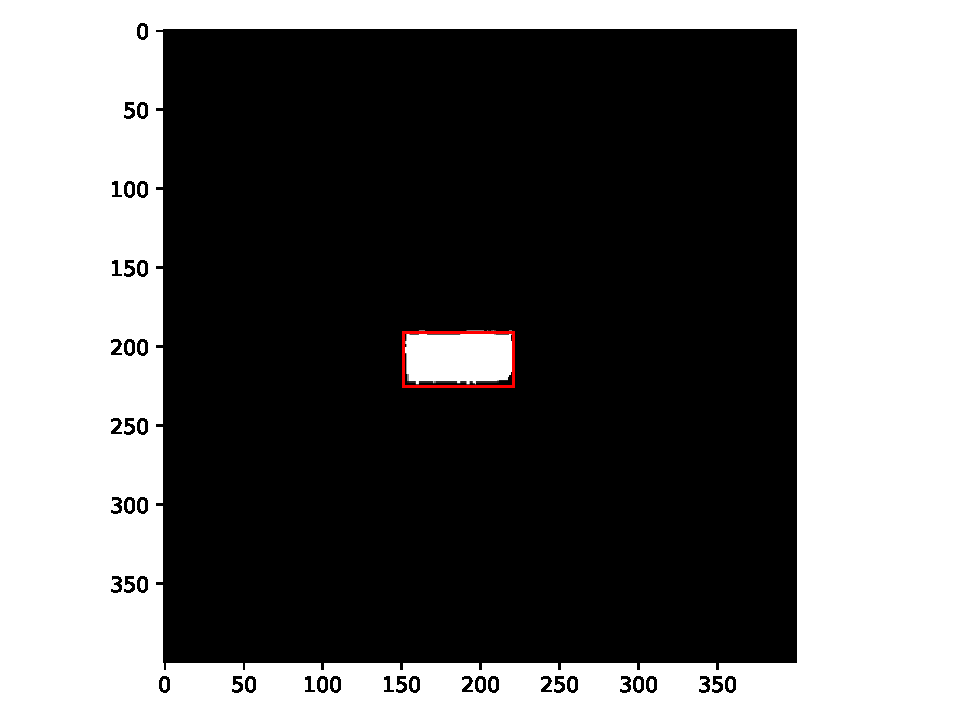
\includegraphics[width=0.9\textwidth]{img/model_demo_5}
    \end{figure}
\end{frame}

\begin{frame}{Resultat}
    \begin{figure}
        \centering
        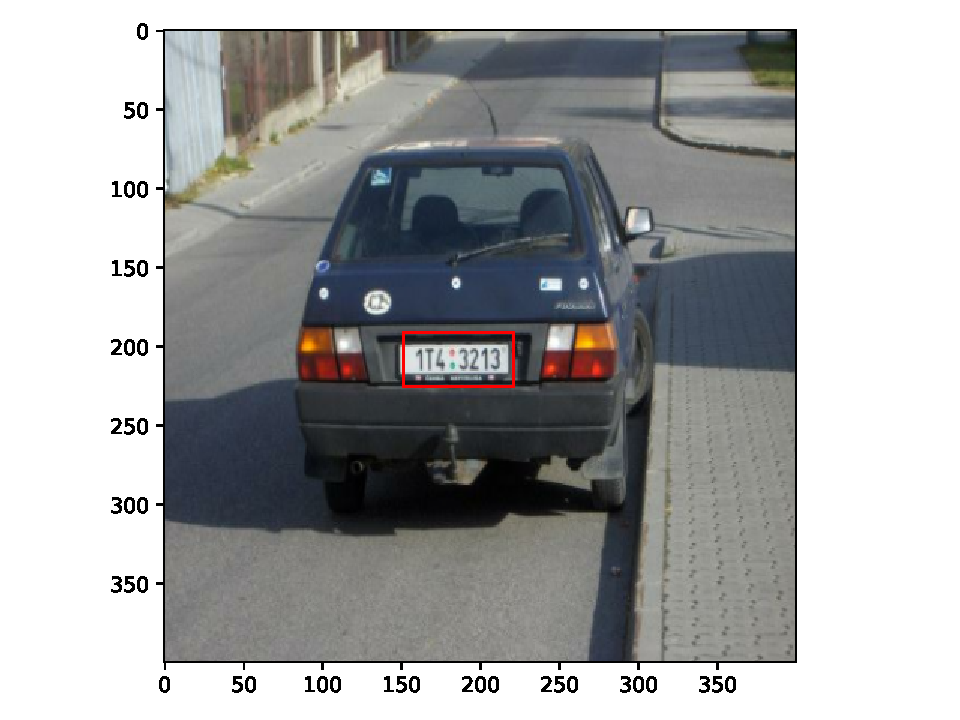
\includegraphics[width=0.9\textwidth]{img/model_demo_6}
    \end{figure}
\end{frame}

\begin{frame}{Details zum Training}
    \textbf{Implementierung in Tensorflow, Training auf Google Colab GPU}
    \begin{itemize}
        \item 534 Zus\"atzliche Trainingsbilder hinzugef\"ugt
        \item Data Augmentation: $949 \Rightarrow 22.776$ Bilder
              \begin{itemize}
                  \item Horizontal Flip, Random Cropping, Random Contrast, Random Brightness
                  \item \textbf{Ben\"otigt >14GB GPU Speicher!}
              \end{itemize}
        \item Gradient Descent mit ADAM Optimizer
        \item Loss: Binary cross entropy
              \begin{equation*}
                  -\sum_{\text{Pixel}} y_{true} \log (y_{pred}) + (1 - y_{true}) \log (1 - y_{pred})
              \end{equation*}
        \item Zur Validierung 20 Bilder aus EU/RO per Hand selektiert
        \item \glqq Early Stopping\grqq{} nach 19 Epochen
    \end{itemize}
\end{frame}
